\chapter{Erkennung der Cry-Units}
\label{sec:vad}

Der erste notwendige Schritt zur Ableitung einer Pain Score aus einem Audiosignal ist die Feststellung, ob in dem Signal überhaupt kindliche Lautäußerungen vorhanden sind. Das Ziel ist, in einem Audiosignal diejenigen Bereiche zu markieren, in denen Stimmaktivität vorhanden ist und daraufhin Beginn und Ende der einzelnen Cry-Units zu festzulegen. Abbildung  \ref{img:vad01} verdeutlicht diese Aufgabe an einem Beispiel: Der obere Graph zeigt in Schwarz ein Audiosignal. Die rote Linie, die das Signal überspannt, zeigt, welche Regionen Stimme enthalten, wobei $1 \hat{=} $ \emph{stimmhaft} (engl. \emph{voiced}) und $0 \hat{=}  $ \emph{nicht stimmhaft} (oder \emph{Stille}, engl. \emph{not voiced}). Das untere Schema zeigt, wie die stimmhaften Signalbereiche zu Cry-Units zusammengefasst wurden.

\begin{figure}[h]
	\centering
	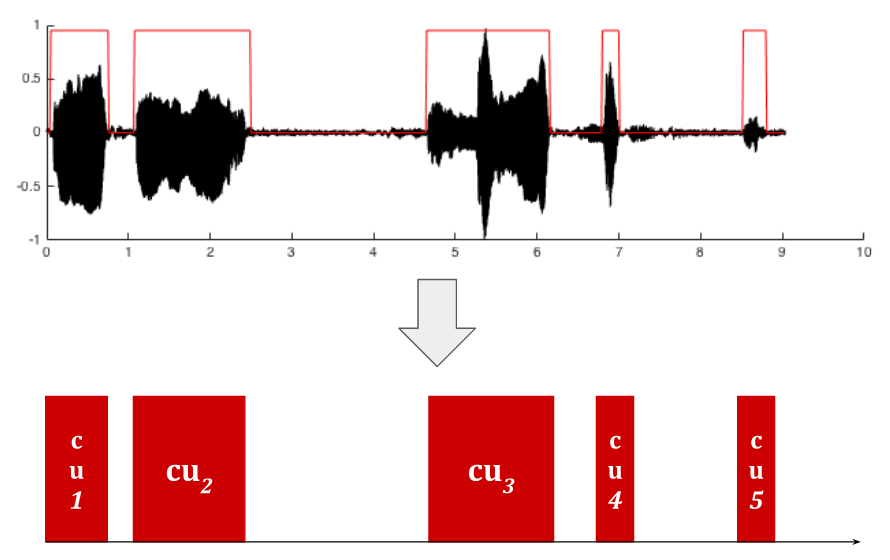
\includegraphics[width=0.7\textwidth]{bilder/vad_introduction02.png}
	\caption{Markierung stimmhafter Bereiche in einem Audiosignal. Oben Schwarz: Das Eingangssignal $x[\;]$. Oben Rot: Klassifizierung in stimmhaft/Stille. Unten Rot: Die fünf erkannten Cry-Units.}
	\label{img:vad01}
\end{figure}

In Kapitel \ref{sec:vad_new} wird die Voice Activity Detection vorgestellt, das Feststellen des Vorhandenseins von Stimme in einem Signal. In Kapitel \ref{sec:marking_cry-units_new} wird besprochen, wie die stimmhaften Signalbereiche zu Cry-Units zusammengefasst werden. In Kapitel \ref{sec:decision_smoothing_new} wird ein Algorithmus vorgestellt, in dem Nachträglich inkorrekt erkannte Anfangs- und Endzeitpunkt von Cry-Units korrigiert werden.

\section{Voice Activity Detection}
\label{sec:vad_new}

\emph{Voice Activity Detection} (kurz \emph{VAD}) oder \emph{Speech Detection} ist bei jeder Art der Sprachverarbeitung von Bedeutung: Im Mobilfunk wird sie beispielsweise eingesetzt, um die Zeitbereiche zu Erkennen, in denen die Teilnehmer sprechen und somit eine Übertragung stattfinden muss. Die größte Herausforderung von VAD-Systemen ist die robuste Erkennung von Stimmaktivität auch bei starkem Hintergrundrauschen. Bis heute wurde keine \glqq perfekte Lösung\grqq{} des Problems gefunden. \cite[S. 1]{vad_granada} \cite[S. 1]{vad_kola} \cite[S. 1]{vad_Lisboa}

Der Grundlegende Aufbau eines VAD-Algorithmus ist wie folgt. Abbildung \ref{img:vad_pipeline} visualisiert diesen Aufbau.
\begin{enumerate}
	\item \textbf{Vorverarbeitung} (engl. Pre-Proccessing) des Signals.
	\item \textbf{Windowing: } Unterteilung des Signals in (einander überlappende) Signalfenster.
	\item \textbf{Extraktion von Eigenschaften} (engl. \emph{Feature-Extraction}) aus jedem Signalfenster.
	\item \textbf{Entscheidung} (engl. \emph{Decision}) über die Präsens oder Abwesenheit von Stimme für jedes Signalfenster auf Grundlage der extrahierten Eigenschaften
	\item \textbf{Decision-Smoothing}, das nachträgliche Hinzufügen oder Entfernen von Entscheidungen mit Hilfe kontextueller Informationen der umliegenden Entscheidungen.\cite[S. 8 - 9]{vad_granada} \cite[S. 1 - 2]{vad_kola}
\end{enumerate}

\begin{figure}[h]
	\centering
	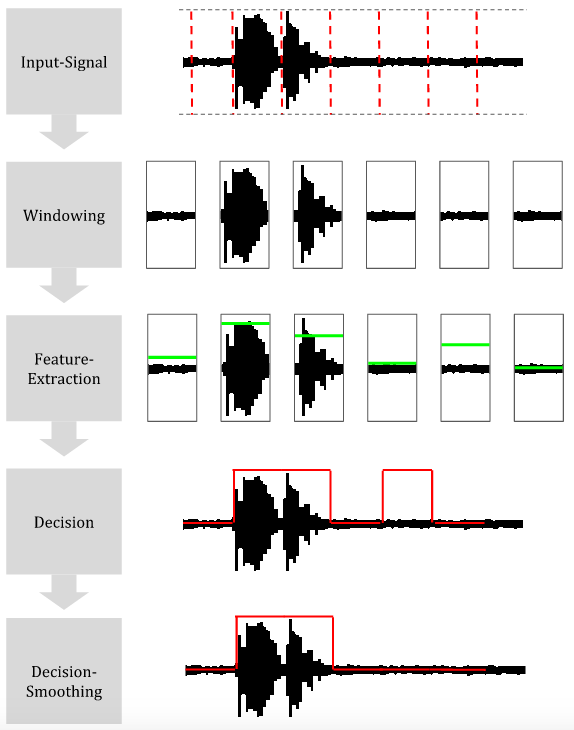
\includegraphics[width=0.65\textwidth]{bilder/vad_pipeline03.png}
	\caption{Aufbau eines VAD-Algorithmus}
	\label{img:vad_pipeline}
\end{figure}


In Kapitel \ref{sec:methods_vad_new} werden die Methoden vorgestellt, die zur Voice Activity Detection erprobt wurden. In Kapitel \ref{sec:vad_study} wird eine Simulationsstudie beschrieben, deren Ziel die Bestimmung derjenigen Methoden war, die sich für die VAD im speziellen Fall kindlicher Lautäußerungen am besten eignen. Kapitel \ref{sec:vad_results} fasst die Ergebnisse zusammen.

\subsection{Methoden}
\label{sec:methods_vad_new}

Die in diesem Kapitel vorgestellten Methoden kombinieren Ideen, die von Moattar et al. \cite{vad_Easy}, Kristjansson et al. \cite{vad_Lisboa}, Waheed et al. \cite{vad_entropy}, Ahmadi et al. \cite{vad_ceps} und Shen et al.\cite{vad_entropie02} vorgestellt wurden.

\subsubsection{Vorverarbeitung}
\label{sec:preprocessing}

Bei der Vorverarbeitung wird das Signal so manipuliert, dass Störeinflüsse auf die darauf folgenden Verarbeitungsschritte minimiert werden. Welche Vorverarbeitung durchgeführt wird, ist Abhängig von der konkreten Aufgabenstellung. Dieser Schritt ist für die VAD optional. So setzten beispielsweise Ahmadi et al. \cite{vad_ceps} einen Bandpassfilter bei der Vorverarbeitung ein, während Moattar et al. \cite{vad_Easy} keine Vorverarbeitung anwendeten. 

In dieser Arbeit sich für eine Vorverarbeitung entschieden, bei der das Signal hinsichtlich seiner Dynamik im Zeitbereich eingeschränkt wird. Dies ist ein typischer Vorverarbeitungsschritt bei Sprachaufnahmen. So wird vermieden, dass ein Signal eventuell zu leise ist, damit überhaupt Etwas darin erkannt werden kann. Einer der hauptsächlichen Gründe, warum ein Signal eine niedrige durchschnittliche Energie aufweisen kann, obwohl es maximal ausgesteuert wurde, sind sehr kurze Pegelspitzen, deren Pegel weit über dem Durchschnittspegel liegen und so eine weitere Erhöhung der Lautstärke verhindern. Da die Audiosignale, die in der in Kapitel \ref{sec:vad_study} vorgestellten Simulationsstudie verwendet wurden, aus inhomogenen Quellen stammen und sehr unterschiedliche Lautstärken hatten, wurde so eine Angleichung der Signalenergien gewährleistet.

Die Dynamikeinschränkung wurde mit Hilfe eines Audio-Kompressors umgesetzt. Dieser verringert Signalspitzen, die über einen festgelegten \emph{Schwellwert} (engl. \emph{Threshold}) $\theta$ liegen, um ein festgelegtes \emph{Verhältnis} (engl. \emph{Ratio)} $\rho$. Ein Schwellwert von $\theta = 0.3$ mit einem Verhältnis von $\rho = 0.5$ bedeutet beispielsweise, dass alle Signalspitzen, die den Wert 0.3 über-, oder $-0.3$ unterschreiten, um 50\% verringert werden. Der Wert eines Samples nach der Kompression $x_{comp}[n]$ ergibt sich somit nach Gleichung \ref{eq:preprocessedX}.

\begin{equation}
\text{comp}(x[n], \theta, \rho) =
\begin{cases}
\theta + (x[n] - \theta) \rho \quad , \text{wenn } x[n] > \theta \\
-\theta + (x[n] + \theta) \rho \quad, \text{wenn } x[n] < -\theta \\
x[n] \quad \text{sonst}
\end{cases}
\label{eq:preprocessedX}
\end{equation}

Die Amplituden hoher Signalspitzen werden so verringert, wodurch Headroom gewonnen wird, welcher anschließend bei der gleichmäßigen Erhöhung aller Amplituden zur Erhöhung der insgesamten Energie genutzt werden kann. Diese Erhöhung kann beispielsweise durch eine Normalisierung nach Gleichung \ref{eq:normalizing} durchgeführt werden.

\begin{equation}
\text{normalize}(x[n]) = \frac{x[n]}{\maxi\{x[\;]\}}
\label{eq:normalizing}
\end{equation}

Bei dem Kompressor, der in dieser Verarbeitungs-Pipeline zur Vorverarbeitung verwendet wird, werden Threshold und Ratio nach Formel \ref{eq:THold} als Funktion des RMS-Wertes des Signals berechnet. Der Parameter $r_a$ gibt den Ziel-RMS-Wert an. Der RMS-Wert wird nach Formel \ref{eq:rms} berechnet.

\begin{equation}
\theta(x[\;]) = \rho(x[\;])  = \bigg[\frac{\text{RMS}(x[\;])}{r_a}\bigg]^{2}
\label{eq:THold}
\end{equation}

Die Vorverarbeitung wurde durchgeführt, indem 1.) die Kompression mit den Parametern nach Gleichung \ref{eq:THold} und 2.) die Normalisierung nach Gleichung \ref{eq:THold} durchgeführt wurde. Abbildung \ref{img:compressing01} zeigt ein Signal vor und nach der Vorverarbeitung nach diesem Prinzip. Um eine zu große Beeinflussung des Signals zu vermeiden, wurde ein Minimalwert für Threshold und Ratio von $0.4$ festgelegt.

\begin{figure}[h]
	\centering
	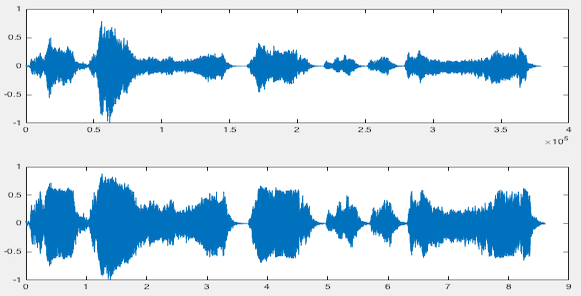
\includegraphics[width=0.7\textwidth]{bilder/compressing01.png}
	\caption{Ergebnis der Vorverarbeitung. Oben: Das Signal vor der Vorverarbeitung. Unten: Das Signal nach der Vorverarbeitung.}
	\label{img:compressing01}
\end{figure}

Diese Vorverarbeitung eignet sich nicht für ein kontinuierliches System, da Samples zur Berechnung des RMS-Wertes mit einbezogen werden, die zu einem Berechnungszeitpunkt in der Zukunft liegen. Das Hauptziel dieser Vorverarbeitung war die Herstellung ähnlicher Energieverhältnisse bei den Signalen, die in der Simulationsstudien in Kapitel \ref{sec:vad_study} verwendet wurden. Damit diese Vorverarbeitung in einem kontinuierlichen System eingesetzt werden kann, wird die folgende Abwandlung vorgeschlagen:
\begin{itemize}
	\item Komplettes Überspringen der Vorverarbeitung, in dem mit Hilfe eines manuell einstellbaren Lautstärkereglers eine ausreichende Signalenergie gewährleistet wird. Würde man beispielsweise anstelle der Analyse des Audiosignals das Gesicht des Neugeborenen mit einer Kamera untersuchen, würde man ebenfalls eine ausreichende Bildhelligkeit voraussetzen.
	\item Die Initialisierung des Kompressor mit \grqq sanften Werten\grqq , wie zum Beispiel $\theta = \rho = 0.7$ und $\maxi\{x[\;] = 0.9\}$. Diese Parameter können nach der Beendigung eines Segmentes (Siehe Kapitel \ref{sec:segmenting}) auf Basis des RMS-Wertes des Segmentes aktualisiert und für die Vorverarbeitung der zukünftigen Werte eingesetzt werden.
\end{itemize}

\subsubsection{Windowing}
\label{sec:windowing}

Angenommen, man führt die Voice Activity Detection für das Signal $x[\;]$ durch und kommt zu dem Schluss, dass in dem Signal (teilweise) Stimme enthalten ist. Ist das Signal mehrere Minuten oder sogar Stunden lang, ist allein aus der Entscheidung nicht ersichtlich, in welchen Zeitbereichen genau Stimme enthalten ist, und in welchen nicht. Um die zeitliche \glqq Auflösung\grqq{} zu erhöhen, wird das Signal in kürzere Zeitfenster zerlegt.

Nach der Vorverarbeitung wird diese Zerlegung mit Hilfe der in Kapitel \ref{sec:stft} als \emph{Windowing} bezeichneten Methode durchgeführt. Das Signal $x[\;]$ wird nach Gleichung \ref{eq:signal-Window} in die Signalfenster $x_0[\;] , \ldots , x_m[\;]$ aufgeteilt. Die Zeitfenster werden zunächst im Zeitbereich belassen. Es wurde sich für die von Waheed et al. \cite{vad_entropy} vorgeschlagene Fensterlänge von \SI{25}{\milli\second} entschieden, als Kompromiss zwischen den von Moattar et al. \cite{vad_Easy} empfohlenen \SI{10}{\milli\second} und den von Ahmadi et al. \cite{vad_ceps} empfohlenen \SI{40}{\milli\second}. Die Fenster überlappen einander um 50\%, das heißt \SI{12.5}{\milli\second}.

Die Entscheidung über das Vorhandensein von Stimme wird \emph{einzeln} für jedes der Signalfenster $x_0[\;] , \ldots , x_m[\;]$ durchgeführt. Grundlage für die Entscheidung ist eine Menge an Features, die für das jeweilige Signalfenster $x_i[\;]$ berechnet wird. Die Erforschung geeigneter Features ist eines der primären Forschungsgegenstände der VAD. In den folgenden Kapiteln \ref{sec:vad_time_features} bis \ref{sec:vad_ceps_features} wird eine Reihe an Features vorgestellt, die in dieser Arbeit zur VAD erprobt wurden. Jedes der in diesen Kapiteln besprochenen Features kann für ein Signalfenster $x_i[\;]$ \`{a} \SI{25}{\milli\second} berechnet werden und als Grundlage für eine Entscheidung dienen. Die Evaluation, welche Eigenschaften sich am besten zur Feststellung von Stimme im speziellen Fall von Neugeborenen eignen, folgt in Kapitel \ref{sec:vad_study}

\subsubsection{Eigenschaften des Zeitbereiches}
\label{sec:vad_time_features}

Im Zeitbereich wurden die beiden Eigenschaften\emph{Root Mean Square} [\emph{RMS}] und \emph{Zero Crossing Rate} [\emph{ZCR}] erprobt.

Moattar et al. \cite{vad_Easy} bezeichnen den Energiegehalt eines Signals als das für die VAD am häufigsten angewandte Attribut. Der RMS-Wert als Feature für ein Signalfenster wurde nach Gleichung \ref{eq:rms} berechnet. Hintergrund ist, dass der Energiegehalt eines Stimmsignals typischerweise höher ist als der des Hintergrundrauschens. Bei geringem Signal/Rausch-Abständen ist diese Bedingung jedoch nicht immer gegeben. Als zweites Attribut des Zeitbereiches wurde die \emph{Zero Crossing Rate} berechnet. Die ZCR nach Formel \ref{eq:zcr} gibt an, wie häufig ein Vorzeichenwechsel im Signal vorkommt. Eine höhere ZCR weist auf ein stimmloses Signal hin, da Rauschen typischerweise eine höhere ZCR als stimmhafte Signale aufweist. Problematisch ist dieses Kriterium bei Signalen, bei denen kein Hintergrundrauschen vorliegt, da sich dort eine ZCR von 0 ergibt.\cite{vad_ceps} Um den Wert in Relation zur Fensterlänge setzen zu können, wurde weiterhin die ZCR durch die Anzahl der Samples eines Signalfensters $N$ geteilt.

\begin{equation}
\text{ZCR}(x_i[\;]) = \sum_{0}^{N-1}|\text{sng}(x_i[n])-\text{sng}(x_i[n-1])|
\label{eq:zcr}
\end{equation}

\subsubsection{Eigenschaften der Autokorrelation}

Neben den in Kapitel \ref{sec:vad_time_features} genannten \glqq einfachen\grqq{} Attributen des Zeitbereiches wurde die Autokorrelation zur VAD erprobt. Die Autokorrelation eignet sich, um Periodizität in einem Signal nachzuweisen. Wie in Kapitel \ref{sec:theVoice} ausgeführt, weisen stimmhafte Signale eine tendenziell stärkeres periodisches Verhalten als das Hintergrundrauschen auf. 

Bei der Autokorrelation wird ein Signal mit einer verzögerten Variante von sich selber korreliert. Gleichung \ref{eq:ACorr} definiert die Autokorrelation des $N$-Sample langen Signalfensters $x_i[\;]$, verzögert um das Lag $k$.

\begin{equation}
\text{A-Corr}_k(x[\;]) = \sum_{n=k}^{N} x[n-k] \cdot x[n]
\label{eq:ACorr}
\end{equation}

Da der Autokorrelationswert neben der Periodizität von der Signalenergie abhängig ist, ist eine Normalisierung des Wertes wünschenswert. Es gibt verschiedene Varianten dieser Normalisierung. Gleichung \ref{eq:NACorr} definiert die \glqq normalisierte Autokorrelation\grqq{}, bei der der Autokorrelationswert durch die RMS-Werte des verzögerten und unverzögerten Signals normalisiert wird.\cite{vad_Lisboa}

\begin{equation}
\text{NA-Corr}_k(x[\;]) = \frac{\sum_{n=k}^{N} x[n-k] \cdot x[n]}{ \sqrt{\sum_{n=1}^{N-k}  x[n]^2}  \cdot  \sqrt{\sum_{n=k}^{N}  x[n]^2} }
\label{eq:NACorr}
\end{equation}

Das Autokorrelations-Signal $a[\;]$ wird erstellt, indem die normalisierte Autokorrelation für verschiedene $k = k_{min} , \ldots , k_{max}$ angewandt wird, wie Gleichung \ref{eq:a-Signal} definiert. 

\begin{equation}
a[\;] := \quad \mathop{\forall}_{k = k_{min}}^{k_{max}} :\ a[k] = \text{NA-Corr}_k(x[\;]) 
\label{eq:a-Signal}
\end{equation}

Ein hoher Wert des Signals $a[\;]$ an der Position $k$ spricht für eine ausgeprägte Periodizität des Signals mit der Frequenz $f =  f_s / k $. Es ist üblich, den Bereich $[k_{min},k_{max}]$ so einzuschränken, dass die Autokorrelation nur für den Frequenz-Raum durchgeführt wird, in dem man Periodizität erwartet.\cite{vad_Lisboa}

In Bezug auf die VAD wurde die Autokorrelation wird als Methode genutzt, um die beiden Attribute \emph{höchste Autokorrelationsspitze} [\emph{aMax}] und \emph{Anzahl der Autokorrelationsspitzen} [\emph{aCount}] zu berechnen. Beide Eigenschaften wurden von Kristjansson et al. \cite[S. 1 - 2]{vad_Lisboa} zur VAD beschrieben. Die \emph{höchste Autokorrelationsspitze} wird in Formel \ref{eq:corrpeak} definiert und bestimmt die höchste Magnitude im Autokorrelationssignal. Ein stimmhaftes Signal hat aufgrund seiner Periodizität erwartungsgemäß einen höheren [\emph{aMax}]-Wert als Rauschen.

\begin{equation}
\text{aMax}(x_i[\;]) = \max_{k}\text{mag}\{\text{NA-Corr}_k(x_i[\;])\}
\label{eq:corrpeak}
\end{equation}

Die \emph{Anzahl der Autokorrelationsspitzen} wird nach Formel \ref{eq:corrcount} berechnet. Das Feature gibt an, wie viele Signalspitzen im Autokorrelationssignal enthalten sind. Rauschen erzeugt höhere [\emph{aCount}]-Wert als stimmhafte Signale, bedingt durch die vielen zufällig entstehenden Periodizitäten.
\begin{equation}
\text{aCount}(x_i[\;]) = \counti_{k}\text{mag}\{\text{NA-Corr}_k(x_i[\;])\}
\label{eq:corrcount}
\end{equation}

Aus Kapitel \ref{sec:acousticModel} ging hervor, dass die Grundfrequenz der Stimme von Neugeborenen zwischen $250$ und $\SI{2000}{\hertz}$ liegt, weshalb auch nur in Lags dieses Bereichs bei der Berechnung beider Features verwendet wurden.

\subsubsection{Eigenschaften des Frequenzbereiches}

Aus dem Frequenzbereich wurden die drei Eigenschaften \emph{unnormalisierte spektrale Entropie} [$SEnt_{u}$], \emph{normalisierte spektrale Entropie}  [$SEnt_{n}$] und \emph{dominanteste Frequenzkomponenten} [$f_{dom}$] erprobt.

Als Vorbereitungsschritt muss das Signalfenster des Zeitbereiches $x_i[\;]$ in den Frequenzbereich $X_i[\;]$ transformiert werden. Die Berechnungsvorschrift ist $X_i[\;] = \text{DFT}\{(w[\;] \cdot x_i[\;])\}$. Wird diese Transformation für alle Signalfenster $x_0[\;], \ldots, x_m[\;]$ eines Signals durchgeführt, entspricht dies der in Kapitel \ref{sec:stft} vorgestellten Short Time Fourier Transformation. Es wurde eine $2048$ Punkte Lange FFT und eine Hamming-Window als Fensterfunktion $w[\;]$ verwendet.

Kristjansson et al. \cite[S. 2]{vad_Lisboa} haben die \emph{spektrale Entropie} zur Voice Activity Detection beschrieben. Dabei wird das Spektrum des Frequenzfensters $X_i[\;]$ als Wahrscheinlichkeitsverteilung betrachtet. Die Entropie als Maß zur \glqq Unreinheit\grqq{} wurde in Kapitel \ref{sec:id3} erläutert. Die \emph{normalisierte spektrale Entropie} wird nach der Formel \ref{eq:norm_se} berechnet. Das Signal $px_i[\;]$ ergibt sich durch die Normalisierung des $N$-Punkte langen Spektrums nach Formel. Bei der normalisierten spektralen Entropie ist zu erwarten, dass Frequenzfenster ohne Stimme einen höheren Wert aufweisen als Fenster mit Stimme.\ref{eq:norm_spek}. 

\begin{equation}
px_i[n] = \frac{X_i[n]}{\sum_{k=1}^{N} X_i[k]}
\label{eq:norm_spek}
\end{equation}

\begin{equation}
\text{SEnt}_n(px_i[\;]) = -\sum_{k=1}^{N}px_i[k] \cdot\log(px_i[k])
\label{eq:norm_se}
\end{equation}

Neben der von Kristjansson et al. \cite{vad_Lisboa} vorgestellten normalisierten spektralen Entropie wurde zusätzlich die \emph{unnormalisierte Spektrale Entropie} nach Formel \ref{eq:unnnorm_se} berechnet. Bei dieser wird das Spektrum nicht normalisiert, das heißt, es gilt $px_i[k] = X_i[k]$. Somit hat die Energie des Signals einen größeren Einfluss den Wert des Attributes. Dabei ist zu erwarten, dass Signalfenster mit Stimme einen höheren Wert aufweisen als Rauschen.\footnote{Kristjansson et al \cite[S. 2]{vad_Lisboa} verwenden zur Entropie-Berechnung den Logarithmus zur Basis 10, anstatt zur Basis 2. Es ist nicht klar, ob es sich dabei um einen Fehler handelt. In dieser Arbeit wurde, wie in dem Paper beschrieben, ebenfalls der Logarithmus zur Basis 10 verwendet!}

\begin{equation}
\text{SEnt}_u(X_i[\;]) = -\sum_{k=1}^{N}X_i[k] \cdot\log(X_i[k])
\label{eq:unnnorm_se}
\end{equation}

In die Berechnungen wurden nur die Frequenzen im Bereich von 250 - \SI{8000}{\hertz} mit einbezogen, da nach Kapitel \ref{sec:acousticModel} die tiefst mögliche Frequenz der Stimme eines Babys bei \SI{200}{\hertz} liegt und nach Shen et al. \cite{vad_entropie02} die Stimme keine Informationen oberhalb von \SI{8000}{\hertz} enthält.

Moattar et al \cite[S. 2550]{vad_Easy} haben die \emph{dominanteste Frequenzkomponente} zur Voice-Activity-Detection vorgestellt. Für jedes Frequenzfenster $X_i[\;]$ wird diejenige Frequenz nach Formel \ref{eq:domfreq} berechnet, welche die höchste Amplitude hat. Es wird dabei, im Gegensatz zur spektralen Entropie, der gesamte Frequenzraum betrachtet. Ein stimmhaftes Signal hat typischerweise eine höhere $f_{dom}$ als ein stimmloses Signal, bedingt durch die hohe Amplitude der Grundfrequenz.

\begin{equation}
f_{dom}(X_i[\;]) = \argmax \{X_i[\;]\}
\label{eq:domfreq}
\end{equation}


\subsubsection{Eigenschaften des Cepstrums}
\label{sec:vad_ceps_features}

Das Cepstrum wird nach Gleichung \ref{eq:cepstrum} als die inverse DFT des Logarithmus des Magnitudensignals des Frequenz-Bereiches definiert.\cite[Cepstral analysis]{ricardo_ceps}

\begin{equation}
c[\;] =  \text{iDFT}\Big\{ \log \Big(\ \big|\ \text{DFT}\{x[\;]\} \big|\ \Big) \Big\}
\label{eq:cepstrum}
\end{equation}	

\begin{figure}[H]
	\centering
	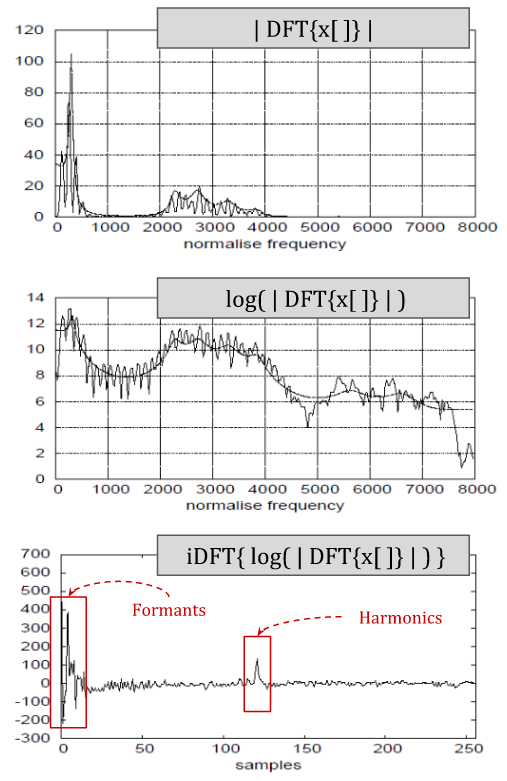
\includegraphics[width=0.6\textwidth]{bilder/cepstrum04.png}
	\caption{Berechnung des Cepstrums. (nach: \cite[Cepstral Analysis, S. 3]{ricardo_ceps})}
	\label{img:cepstrumOverview}
\end{figure}

Das Vorgehen wird mit Hilfe des Beispiels aus Abbildung \ref{img:cepstrumOverview} erläutert. $ |\ \text{DFT}\{x[\;]\} \big| $  zeigt das Spektrum eines \glqq typischen stimmhaften\grqq{} Signals $x[\;]$. Es sind die in Kapitel \ref{sec:theVoice} erläuterten für ein stimmhaftes Signal typischen harmonischen Obertöne zu sehen, welche mit steigender Frequenz an Amplitude verlieren. Durch das logarithmieren des Spektrums $\log \Big(\ \big|\ \text{DFT}\{x[\;]\} \big|\ \Big)$ wird die Dynamic des Frequenzbereiches verringert und somit der Amplitudenverlust der höheren Obertöne verringert. Nun stellt man sich vor, dieses Spektrum wäre ein Signal des Zeitbereiches. Dieses Signal würde man als ein annährend periodisches Signal mit einer Amplituden-Modulation interpretieren, das heißt ein Signal mit hoher Frequenz, addiert mit einem Signal mit nierdiger Frequenz. Um diese beiden Komponenten voneinander zu trennen, müsste man eine weitere DFT anwenden. Diese DFT kommt in dem Fall einer inversen DFT gleich, da das Phasen-Signal verworfen wurde. Man erwartet in diesem \glqq Spektrum vom Spektrum\grqq{} einen Peak im \glqq oberen Frequenzbereich\grqq , bedingt durch die harmonischen Oberwellen, sowie einen Peak im \glqq unteren Frequenzbereich\grqq, bedingt durch die Formanten.\cite[Cepstral analysis]{ricardo_ceps}

Der Bereich dieser \glqq Fouriertransformation der Fouriertransformation\grqq{} wird als \emph{Cepstrum} bezeichnet. Cepstrum ist ein ein Wortspiel, welches durch die Umkehrung der ersten vier Buchstaben des Wortes "Spectrum" entsteht. Die Unabhängige Variable des Cepstrum wird als \emph{Quefrency} bezeichnet. Damit wird verdeutlicht, dass die unabhängige Variable des Cepstrum zwar mathematisch betrachtet die Zeit darstellt, jedoch als Frequenz interpretiert wird.\cite[S. 7]{ricardo_ceps}

\begin{figure}[h]
	\centering
	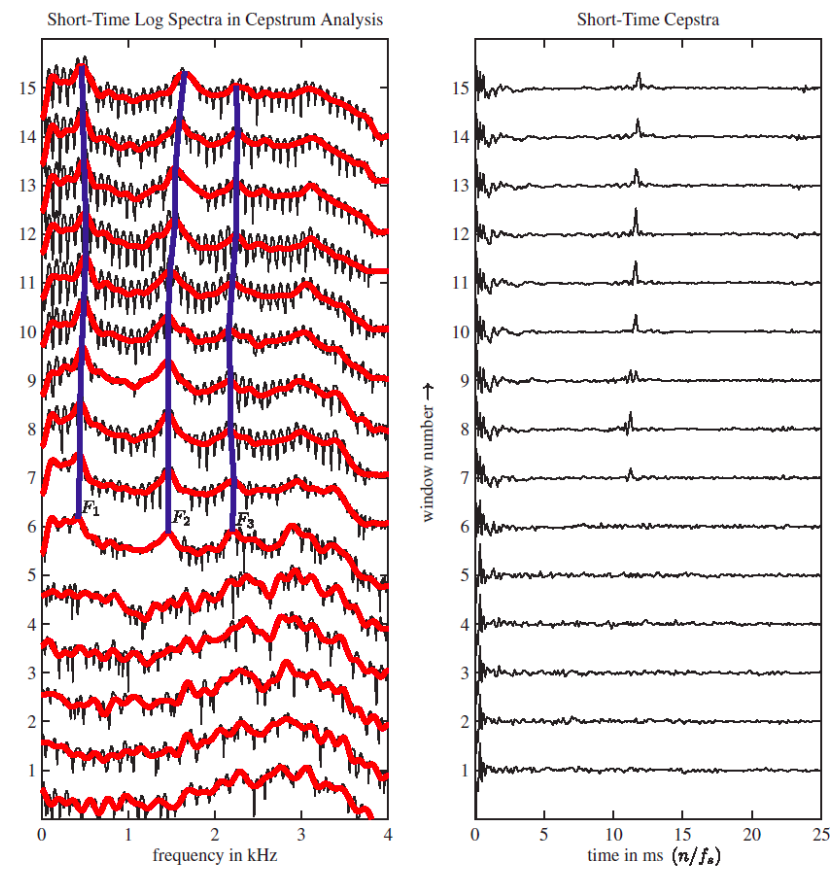
\includegraphics[width=0.6\textwidth]{bilder/cepstrum05.png}
	\caption{Aufkommen eines Peaks im oberen Quefrency-Bereich bei stimmhaften Signalfenstern. \cite[Cepstral Analysis, S. 17]{ricardo_ceps}}
	\label{img:cepstrumVoicedPeak}
\end{figure}	

Ein Auftauchen eines Peaks im oberen Quefrency-Bereich $> \SI{3}{\milli\second}$ spricht für das Vorhandensein von harmonischen Obertönen im Signal, wie sie durch Stimme erzeugt werden. Abbildung \ref{img:cepstrumVoicedPeak} verdeutlicht das Prinzip an einem Beispiel. Zu sehen ist die STFT eines Signals mit einer Fensterlänge von $\SI{50}{\milli\second}$ und einer Hopsize von $\SI{12.5}{\milli\second}$. Links wird das logarithmierte Spektrum abgebildet, rechts das Cepstrum. Die Frames 1 bis 5 sind stimmlos, die Frames 8 bis 15 sind stimmhaft, und die zwischen-Frames eine Mischung. Man sieht das Aufkommen eines Peaks bei einer Quefrency $q = \SI{12}{\milli\second}$.\cite[S. 16]{ricardo_ceps}

Abbildung \ref{img:cepstrumPitch} verdeutlicht, wie eine Grundfrequenz $f_0$ im Zeitbereich einen Peak im Cepstrum erzeugt. So weist ein Peak an bei der Quefrency $q$ auf eine Grundfrequenz von $f_0 = f_s/q$ hin.\cite{cepstrumPitchTranslation}

\begin{figure}[h]
	\centering
	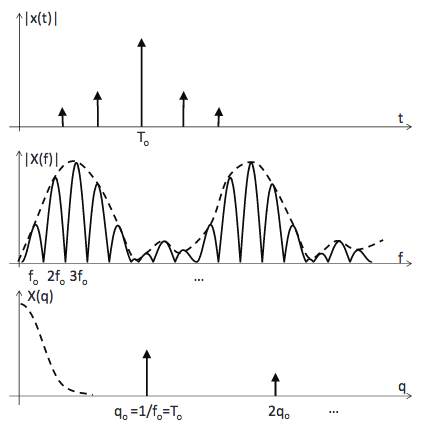
\includegraphics[width=0.6\textwidth]{bilder/cepstrumPitch.png}
	\caption{Feststellung der Grundfrequenz aus dem Cepstrum. \cite{cepstrumPitchTranslation}}
	\label{img:cepstrumPitch}
\end{figure}

In Bezug auf die Voice Activity Detection wurde das Cepstrum genutzt, um die beiden Features \emph{Obere Cepstrum-Spitze} [$Ceps_{mag}$] und \emph{Quefrency der oberen Cepstrum-Spitze} [$Ceps_{loc}$] zu berechnen.

Ahmadi et al. \cite{vad_ceps} sowie Kristjansson et al.\cite{vad_Lisboa} schlagen vor, die Höhe der Magnitude eines Peaks im oberen Bereich des Cepstrums als Maß für die Stimmhaftigkeit des Signals einzusetzen. Formel \ref{eq:ceps_maxpeak} definiert die Berechnung. $c_i[\;]$ ist das Cepstrum des $i$-ten Frequenzfensters $X_i[\;]$. Wie in Kapitel \ref{sec:acousticModel} erläutert, liegt die Grundfrequenz bei kindlichen Lautäußerungen zwischen 200 und \SI{2000}{\hertz}, was einem Quefrency-Bereich von 5 - \SI{40}{\milli\second} entspricht. Folglich werden bei der Berechnung nach Formel \ref{eq:ceps_maxpeak} nur Quefrency-Werte in diesem Bereich betrachtet. 

\begin{equation}
Ceps_{mag}(c_i[\;]) = \maxmagi_{q = q_{min} \ldots , q_{max}}\{ \; c[q] \; \}
\label{eq:ceps_maxpeak}
\end{equation}

Als zweites Attribut, welches auf dem Cesptrum basiert, wurde die Quefrency der höchsten Amplitude des oberen Cepstrum-Bereiches nach Formel \ref{eq:ceps_loc} berechnet. Bei Signalfenstern ohne Stimme ist es wahrscheinlicher, dass sich die höchste Amplitude am Mindest- oder Maximalwert des durchsuchten Quefrency-Bereiches befindet.

\begin{equation}
Ceps_{loc}(c_i[\;]) = \argmax \{ \; c[\;] \; \}
\label{eq:ceps_loc}
\end{equation}	

\subsubsection{Differenz-Feature}
\label{sec:vad_dif_feature}

Abbildung \ref{img:vadAllFeatures} visualisiert alle Attribute, die in den Kapiteln \ref{sec:vad_time_features} bis \ref{sec:vad_ceps_features} vorgestellt wurden. Der oberste Plot zeigt das Audiosignal aus Abbildung \ref{img:vad01} mit einem Signal/Rausch-Abstand von \SI{20}{\decibel}. Der rote Graph über dem Plot klassifiziert die Zeitbereiche in $1 \; \hat{=} $ \emph{stimmhaft} und $0 \; \hat{=}$ \emph{nicht stimmhaft}. Alle darunter liegenden Plots zeigen den zeitlichen Verlauf der entsprechenden Attribute.

\begin{figure}[h]
	\centering
	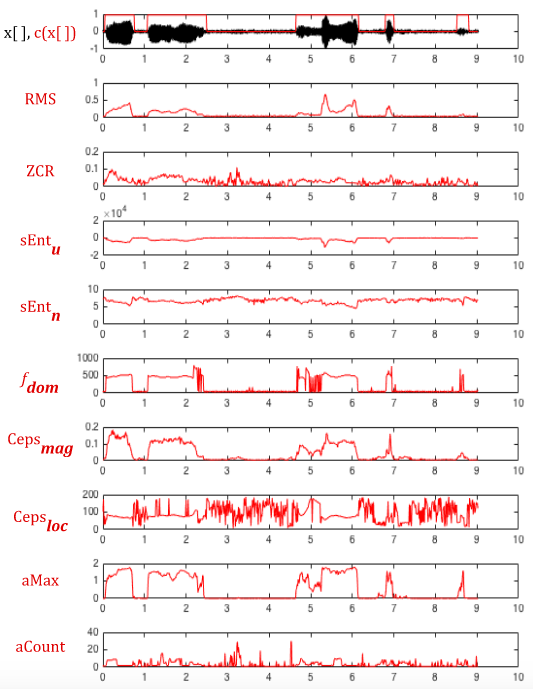
\includegraphics[width=0.85\textwidth]{bilder/allFeatures01.png}
	\caption{Übersicht über alle Features, die für die Voice Activity Detection erprobt wurden.}
	\label{img:vadAllFeatures}
\end{figure}

Abbildung \ref{img:min-signal} zeigt den zeitlichen Verlauf des RMS-Features im Detail. (A) zeigt das verhalten des \emph{RMS}-Attributes bei einem Signal/Rauschabstand von \SI{50}{\decibel}. Die stimmlosen Zeiträume haben einen weitaus niedrigeren RMS-Wert als die Zeiträume mit Stimme. In (B) ist das selbe Signal mit einem Signal/Rauschabstand von \SI{3}{\decibel} zu sehen. Nun liegen die RMS-Werte der stimmlosen Bereiche nur noch knapp unter denen des Sprachsignals. Zu sehen ist, dass starkes Hintergrundrauschen ähnlich hohe Feature-Werte erzeugen kann wie die Stimme.

\begin{figure}[h]
	\centering
	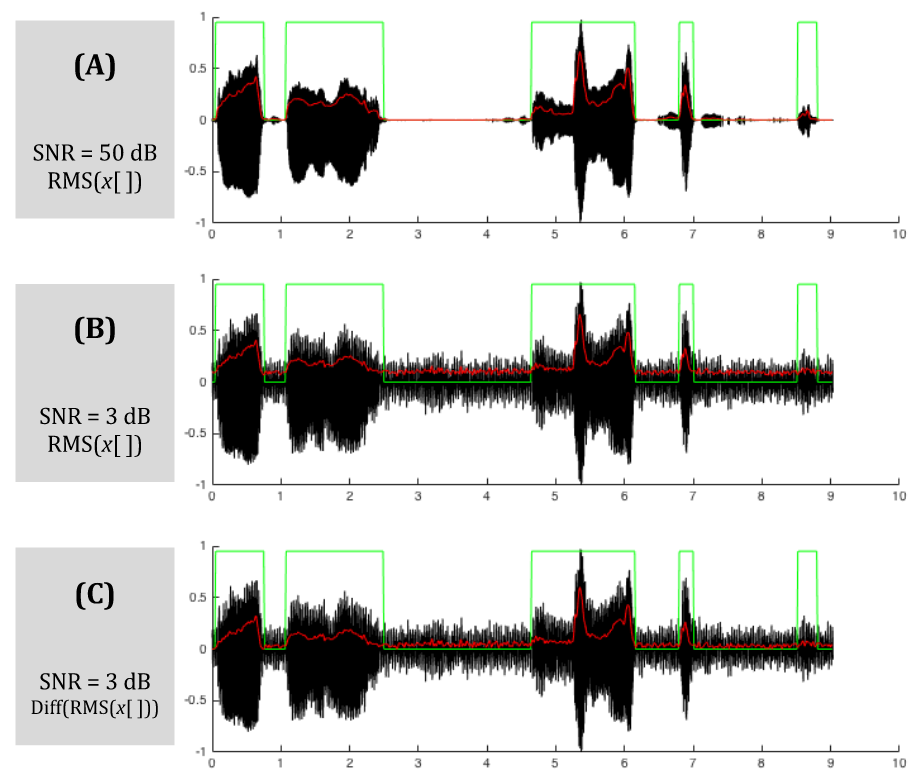
\includegraphics[width=0.7\textwidth]{bilder/rms_diff.png}
	\caption{Das RMS-Feature bei verschiedenen Signal/Rausch-Abständen. Schwarz: Eingangs-Signal $x[\;]$. Grün: Klassifizierung in Stimmhaft/Stille. Rot: Feature-Wert.}
	\label{img:min-signal}
\end{figure}

Moattar et al \cite{vad_Easy} und Waheed et al \cite{vad_entropy} präsentierten die Idee, den Wert des jeweiligen Attributes zu messen, der in den stimmlosen Bereichen durch das Hintergrundrauschen erzeugt wird. Es kann davon ausgegangen werden, dass die ersten Signalfenster eines Signals stimmlos sind, und der Feature-Wert des Rauschens somit anhand dieser Fenster bestimmt werden kann. Bei einer langanhaltenden und kontinuierlichen Analyse können sich sowohl der Signal/Rausch-Abstand als auch die Qualität des Rauschens ständig ändern, weshalb die von den stimmlosen Bereichen erzeugten Attributwerte regelmäßig aktualisiert werden müssen. Es kann weiterhin davon ausgegangen werden, dass die Länge einer Cry-Unit eine bestimmte Länge $t_{max}$ nicht überschreiten kann, bevor das Baby Luft holen muss und somit zumindest ein stimmloses Zeitfenster entsteht, welches das Hintergrundrauschen enthält. Zeskind et al. \cite[S. 325]{rythmic} haben $t_{max} = \SI{4.75}{\second}$ bestimmt. In einem Zeitbereich $ t > t_{max}$ muss somit zumindest ein Feature-Wert enthalten sein, der durch stimmlose Signalteile erzeugt wird. 

Auf Basis dieser Überlegung wurde das \emph{Differenz-Feature} Diff\textsubscript{t}(\text{Feat}$(x_i[\;])$) nach Formel \ref{eq:difFeature} definiert als die Differenz zwischen einem aktuell gemessenen Attributwerte und dem geringsten Attributwerte, welcher im vergangenen Zeitbereich $t$ gemessen wurde. Feat$(x_i[\;])$ bezeichnet dabei einen beliebigen Feature-Wert des Signalfensters $x_i[\;]$, $t_{xi}$ die Länge eines Signalfensters in Sekunden (in diesem Fall \SI{25}{\milli\second}), und $t$ der in der Vergangenheit zu durchsuchende Zeitbereich in Sekunden $> t_{max}$. In Abbildung \ref{img:min-signal} wird in (C) das Differenz-Feature für den RMS-Wertes gezeigt.

\begin{equation}
\text{Diff}_t(\text{Feat}(x_i[\;])) = \text{Feat}(x_i[\;])\ - \mini_{k=i-z...i}\{\text{Feat}(x_k[\;])\}, \qquad z = \frac{2 \cdot t}{t_{xi}}
\label{eq:difFeature}
\end{equation}

In dieser Arbeit wurde $t = \SI{5}{\second}$ festgelegt. Es ist zu beachten, dass die Attribute \emph{ZCR, SEnt\textsubscript{u}} und \emph{aCount} zur Berechnung des Differenz-Features bezüglich ihres Vorzeichens invertiert werden müssen, da bei Ihnen ein niedriger an Stelle eines hohen Wertes stimmhafte Signale anzeigen. Das einzige Attribut, für dass die Berechnung des Differenz-Features keinen Sinn macht, ist das \emph{Ceps\textsubscript{loc}}-Attribut, da es bei stimmlosen Signalabschnitten sowohl einen höheren als auch einen niedrigeren Wert annehmen kann.

\subsubsection{Entscheidung}

Die einfachste Variante, um zu Entscheiden, ob ein Signalfenster $x_i[\;]$ stimmhaft ist, ist, eines der vorgestellten Features als Entscheidungsgrundlage zu wählen und einen festen Grenzwert $\theta$ festzulegen, bei dessen Über- oder Unterschreitung das Fenster als stimmhaft klassifiziert wird. Die Entscheidung lässt sich als Klassifizierungsfunktion $C$ definieren, welche ein Signalfenster abbildet auf $Y = \{ 1 \; \hat{=} \; \text{stimmhaft}, 0 \; \hat{=} \; \text{nicht stimmhaft}\}$, das heißt $C(x[\;]) \mapsto \{1,0\}$. Die Klassifizierungsfunktion nimmt dann die folgende Form an:

\begin{equation}
	C(x_i[\;]) = 
\begin{cases}
1 \quad , \text{wenn Feat}(x_i[\;]) > \theta \\
0 \quad , \text{sonst}
 \end{cases}
\end{equation}

 Abbildung \ref{img:thresholded} verdeutlicht das Prinzip an einem Beispiel. Das Feature, dass als Entscheidungsgrundlage genutzt wird, ist der \emph{RMS}-Wert. Ein Grenzwert von $\theta = 0.18$ würde in diesem Fall eine weitestgehend richtige Klassifizierung gewährleisten.

\begin{figure}[h]
	\centering
	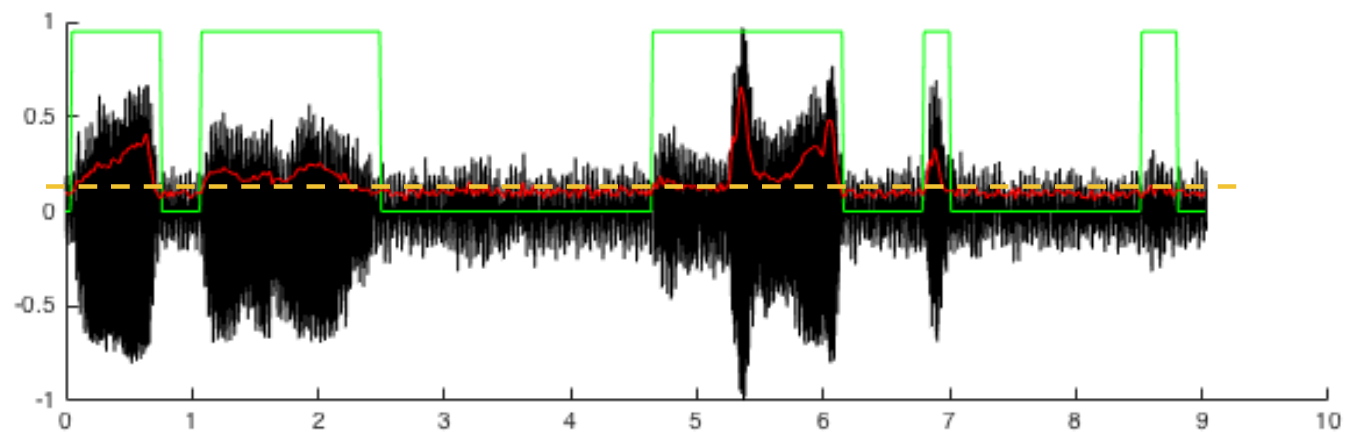
\includegraphics[width=0.6\textwidth]{bilder/thresholded02.png}
	\caption{Thresholding eines Features. Schwarz: Das Eingangssignal $x[\;]$. Grün: Klassifizierung in Stimmhaft/Stille. Rot: RMS-Feature. Orange: Grenzwert}
	\label{img:thresholded}
\end{figure}

Die Frage ist, wie man diesen Grenzwert findet. In einigen Veröffentlichungen, so wie der von Moattar et al. \cite{vad_Easy} wird empfohlen, den Grenzwert experimentell festzustellen. In dieser Arbeit wurde sich für den Ansatz einer automatisierten, datengetriebenen Suche der Grenzwerte mit Hilfe des in Kapitel \ref{sec:id3} vorgestellten \emph{C4.5}-Algorithmus entschieden. Der Grundgedanke ist wie folgt: Angenommen, man hat einen Trainingsdatensatz zur Verfügung, bestehend aus einer Menge an Signalen mit Aufnahmen von kindlichen Lautäußerungen, in denen manuell die stimmhaften Signalabschnitte markiert wurden. Diese Signale zerlegt man nach den besprochenen Methoden in kürzere Signalfenster und berechnet für jedes Signalfenster das Feature, dessen Grenzwert man sucht. Jedem Signalfenster versieht man außerdem mit dem Klassenlabel $y \in Y$ auf Basis der manuellen Markierungen. Ein \emph{Signalfenster} $x_i[\;]$ wird so zu einem \emph{Example} $e_i = (\text{Feat}(x_i[\;]), y_i)$. Nun kann der \emph{C4.5}-Algorithmus verwendet werden, um für das Feature den Grenzwert zu finden, der für diese Datenbasis die Klassifizierung mit der höchsten Genauigkeit vornimmt. Voraussetzung dafür ist, dass der \emph{C4.5}-Algorithmus gezwungen wird, einen Entscheidungsbaum mit einer maximalen Tiefe von $1$ zu erzeugen, damit auch nur ein Grenzwert gesucht wird. Ist das Feature, für das der Grenzwert gesucht wird, ein Differenz-Feauture (siehe Kapitel \ref{sec:vad_dif_feature}), so lässt sich dieser Grenzwert als ein adaptiver Grenzwert interpretieren, der sich an den aktuellen SNR anpasst.

Die Verwendung des \emph{C4.5}-Algorithmus bringt die Möglichkeit mit sich, eine beliebige Menge an Features in die Klassifizierung mit einzubeziehen. Die Klassifizierung muss also nicht zwingend auf Grundlage nur eines Attributes geschehen. Angenommen, es werden die beiden Features Ceps$_{mag}$ und der RMS-Wert für jedes Signalfenster berechnet. Der \emph{C4.5}-Algorithmus würde nun für einen Trainingsdatensatz einen Entscheidungsbaum konstruieren, bei dem durch das hierarchische Setzen von Grenzwerten die Klassifikation vorgenommen wird. Listing \ref{lst:tree01} zeigt ein Beispiel für eine so resultierende, fiktive Klassifizierungsfunktion.

\begin{lstlisting}[frame=single,mathescape=true,basicstyle=\footnotesize,language=Java,label=lst:tree01,caption=Beispiel eines CART-Entscheidungsbaums,linewidth=1\textwidth]
if Ceps$_{mag}$($x_i[\;]$) > 0.2
|   if RMS($x_i[\;]$) < 0.13
|   |   C($x_i[\;]$) = 0
|   |else
|   |   C($x_i[\;]$) = 1
|else
|    C($x_i[\;]$) = 1
\end{lstlisting}

Wird dem \emph{C4.5}-Algorithmus eine größere Menge an Attributen zur Verfügung gestellt, auf deren Basis der Klassifikator entworfen wird, wird der Entscheidungsbaum implizit zeigen, welche Features für die VAD besser geeignet sind, da sie höher im Entscheidungsbaum stehen werden. Es besteht jedoch die Gefahr, dass der Klassifikator in ein lokales Maximum gelaufen ist und eine suboptimale Auswahl an Features durch den Algorithmus getroffen wurde. Außerdem besteht die Gefahr von Overfitting, insofern Entscheidungsbäume mit beliebiger Tiefe zugelassen werden.

\subsection{Simulations-Studie}
\label{sec:vad_study}

In Kapitel \ref{sec:methods_vad_new} wurde eine Übersicht über die Methoden gegeben, die in dieser Arbeit zur Voice Activity Detection erprobt und/oder eingesetzt wurden. Neben Methoden zur Vorverarbeitung und zum Windowing wurde eine Reihe an Features vorgestellt, die für ein Signalfenster als Entscheidungsgrundlage für die Erkennung von Stimme dienen können. Schlussendlich wurde argumentiert, wie der \emph{C4.5}-Algorithmus genutzt werden kann, um einen Klassifikator zu entwerfen, der die Entscheidung über das Vorhandensein von Stimme in einem Signalfenster auf Grundlage einer Menge von Features fällt. Dafür wird ein Datensatz zum Training des \emph{C4.5}-Algorithmus benötigt.

Das Ziel ist es nun, auf Grundlage dieser Methode den tatsächlichen Klassifikator zu finden. Der Klassifikator soll dabei die folgenden Bedingungen erfüllen:

\begin{itemize}
\item Der Klassifikator soll eine möglichst kleine Anzahl an Features verwenden, da es zu aufwendig ist, alle vorgestellten Features nur für die VAD in einem kontinuierlichen System zu berechnen.
\item Der Klassifikator soll eine möglichst hohe Genauigkeit erzielen, unabhängig von Stärke und Qualität des Hintergrundrauschens.
\end{itemize}

Das Vorgehen zum finden des Klassifikators war wie folgt:
\begin{enumerate}
\item Es wurde ein Menge an Trainingsdatensätzen erstellt, indem ...
	\begin{enumerate}[label*=\arabic*.]
	\item ... in einer Menge an Audioaufnahmen weinender Babys manuell die stimmhaften Signalabschnitte markiert wurden,
	\item ... die Signale vorverarbeitet, in Signalfenster zerlegt und für jedes Signalfenster alle vorgestellten Features berechnet wurden,
	\item ... woraus Datensätze erzeugt wurden, wobei jeder Datensatz nur eine bestimmte Untermenge der Features zur Verfügung gestellt bekam.
	\end{enumerate}
\item Auf Basis jedes Datensatzes wurde mit Hilfe des \emph{C4.5}-Algorithmus ein Klassifikator erzeugt.
\item Jeder Klassifikator wurde bezüglich seiner Genauigkeit gegen eine Menge an Trainingsdatensätze unterschiedlicher Signal/Rausch-Abstände evaluiert.
\item Schlussendlich wurde sich für einen Klassifikator auf Grundlage der Evaluationsergebnisse entschieden.
\end{enumerate}

In Kapitel \ref{sec:vad_database} wird die Erstellung des Datensatzes erläutert. In Kapitel \ref{sec:vad_training} wird das Vorgehen beim Training des \emph{C4.5}-Algorithmus ausgeführt, und in Kapitel \ref{sec:vad_results} die Ergebnisse ausgewertet.

\subsubsection{Erstellung der Datensätze}
\label{sec:vad_database}

Der zeitliche Rahmen dieser Arbeit ermöglichte es nicht, selber Audioaufnahme von Babys zu machen. Daher wurden sechs Audioaufnahmen mit dem Weinen verschiedener Babies unterschiedlicher Qualität und Intensität von der freien Online-Sound-Bibliothek \url{https://www.freesound.org/} heruntergeladen und zu Segmenten \`{a} \SI{10}{\second} beschnitten. Es handelt sich um weitestgehend rauschfreie Aufnahmen, die von verschiedenen Babys stammen. In den Audiosignalen wurden manuell die Zeitbereiche markiert, welche Stimme enthalten.\footnote{Es wurden \emph{keine} Geräusche markiert, bei denen es sich offensichtlich um Einatmungs-Geräusche handelt. Geräusche, bei denen nur Anhand der Aufnahme nicht mit Sicherheit festgestellt werden konnte, ob es sich um Einatmungs- oder Ausatmungsgeräusche handelt, wurden als Stimme markiert. Die Begründung liegt darin, dass nach Varallyay \cite{cry_thesis} bei der Einatmung entstehenden Geräusche keine verwertbare Information enthalten. }

Weiterhin wurden drei verschiedene Rauschsignale heruntergeladen. Es handelt sich um \glqq realistische\grqq{} Atmosphären von Krankenhäusern. Jedes der sechs Audioaufnahmen der Babys wurde mit jedem der drei Rauschsignale überlagert, einmal mit einem Signal/Rausch-Abstand von \SI{50}{\decibel} (\glqq fast unhörbares Rauschen\grqq), und einmal mit einem Signal/Rausch-Abstand von \SI{3}{\decibel} (\glqq starkes Rauschen\grqq). Außerdem wurde ein siebte Aufnahme eines Babys heruntergeladen, welches mit einem vierten Rauschsignal mit einem SNR von \SI{7}{\decibel} überlagert wurde. Dieses Signal spielte eine Sonderrolle, da es nur zur Verifikation verwendet wurde. 

So wurden vier Mengen an Audiosignalen $\boldmath{A_{\text{SNR}}}$ erzeugt:

\begin{description}
	\item[$\boldmath{A_{\SI{50}{\decibel}}}$] enthält $3 \cdot 6 = 18$ Audiosignale, wobei jedes der sechs Baby-Aufnahmen mit jedem der drei Rauschsignale bei einem Signal/Rausch-Abstand von \textbf{\SI{50}{\decibel}} überlagert wurde.

	\item[$\boldmath{A_{\SI{3}{\decibel}}}$] enthält $3 \cdot 6 = 18$ Audiosignale, wobei jedes der sechs Baby-Aufnahmen mit jedem der drei Rauschsignale bei einem Signal/Rausch-Abstand von \textbf{\SI{3}{\decibel}} überlagert wurde.
	
	\item[$\boldmath{A_{50+\SI{3}{\decibel}}}$] $ = \{ A_{\SI{50}{\decibel}} \cup  A_{\SI{3}{\decibel}}\} = 32$ Audiosignale
	
	\item[$\boldmath{A_{\SI{7}{\decibel}*}}$] enthält ein Audiosignal, bei dem eine siebte Aufnahme eines Babys mit einem vierten Rauschsignal bei einem Signal/Rausch-Abstand von \textbf{\SI{7}{\decibel}} überlagert wurde
	
\end{description}

Aus diesen Audiosignalen wurden die tatsächlichen Datensätze $\boldmath{D_{\text{SNR,Feats}}}$ nach dem folgenden Vorgehen erzeugt:

\begin{enumerate}
\item Jedes der Signale wurde nach dein Kapitel \ref{sec:preprocessing} vorgestellten Methoden vorverarbeitet und in Signalfenster \`{a} \SI{25}{\milli\second} zerlegt.
\item Jedes Signalfenster $x_i[\;]$ wurde zu ein Example $e_i$ gewandelt, in dem eine bestimmte Untermenge der vorgestellten Features für das Signalfenster berechnet wurde. Tabelle \ref{tab:vad_feat_subsets} gibt eine Übersicht über die insgesamt 9 Untermengen. Die ersten vier Untermengen beinhalten jeweils die Features, die sich durch die jeweilige Methoden erzeugen lassen. Die nächsten fünf Untermengen enthalten jede mögliche paarweise Kombination der ersten vier Untermengen, mit Ausnahme des Cepstrum+Autokorrelation, da die Features dieser Bereiche am rechenaufwendigsten sind. Jedem Example wurde das entsprechende Klassenlabel beigefügt.

\begin{table}[h]
\centering
\caption{Übersicht über die gebildeten Feature-Untermengen}
\label{tab:vad_feat_subsets}
\begin{tabular}{@{}ll@{}}
\toprule
\multicolumn{1}{c}{Name} & verwendete Features                                                              \\ \midrule
Zeit                     & RMS, Diff(RMS), ZCR, Diff(-ZCR)                                                  \\
Spektrum                 & SEnt$_u$, Diff(SEnt$_u$), SEnt$_n$, Diff(-SEnt$_n$), $f_{dom}$, Diff(f\_\{dom\}) \\
Autokorr.                & aMax, Diff(aMax), aCount, Diff(-aCount)                                          \\
Cepstrum                 & Ceps$_{mag}$, Diff(Ceps$_{mag}$), Ceps$_{loc}$                                   \\
Zeit+Spektrum            & RMS, \ldots , SEnt$_u$, \ldots                                                   \\
Zeit+Autokorr.           & RMS, \ldots , aMax, \ldots                                                       \\
Zeit+Cepstrum            & RMS, \ldots , Ceps$_{mag}$, \ldots                                               \\
Spek.+Autokorr.          & SEnt$_u$, \ldots , aMax , \ldots                                                 \\
Spek.+Cepstrum           & SEnt$_u$, \ldots, Ceps$_{mag}$ ,\ldots                                           \\ \bottomrule
\end{tabular}
\end{table}
\item Alle Examples, die aus der selben Signalmenge $\boldmath{A_{\text{SNR}}}$ stammen und die selbe Feature-Untermenge teilen, werden in einem Datensatz $\boldmath{D_{\text{SNR,Feats}}}$ zusammengefasst. Beispielsweise enthält der Datensatz $\boldmath{D_{\SI{50}{\decibel},\text{Zeit}}}$ alle Examples, die auf Grundlage der Signalmenge mit einem Signal/Rausch-Abstand von \SI{50}{\decibel} unter Verwendung der in Tabelle \ref{tab:vad_feat_subsets} aufgelisteten Features des Zeitbereiches erzeugt wurden.
\item Da in allen Datensätzen rund dreimal mehr Positives (das heisst, Examples aus stimmhaften Signalfenstern) enthalten waren als Negatives, wurde jedes in einem Datensatz enthaltene Negative dreimal eingefügt. So wurde ein ausgewogenes Verhältnis an Positives und Negatives gewährleistet.
\end{enumerate}

Auf diese Art und Weise wurden aus den vier Signalmengen $\boldmath{A_{\SI{50}{\decibel}}}, \ldots , \boldmath{A_{\SI{7}{\decibel}*}}$ und den 9 Feature-Untermengen insgesamt $4 \cdot 9 = 36$ \emph{Trainingsdatensätze} $\boldmath{D_{\text{SNR,Feats}}}$ gebildet. Wird einer dieser Datensätze als Testdatensatz verwendet, so sind die Features des Datensatzes unerheblich, da nur die Informationen der Klassenlabels beim Testing benötigt werden. Ein Testdatensatz $\boldmath{D_{\text{SNR}}}$ kann also erzeugt werden, in dem bei einem beliebigen Trainingsdatensatz mit dem Entsprechenden SNR die Featureinformationen ignoriert werden.

\subsubsection{Training und Evaluation}
\label{sec:vad_training}

Das Ziel war es nun, auf Basis der Datensätze durch den \emph{C4.5}-Algorithmus denjenigen Klassifikator zu finden, der für sowohl niedrige als auch hohe SNRs eine möglichst hohe Klassifikationsgenauigkeit erzielt. Es ist beispielsweise denkbar, dass ein Klassifikator, welcher auf Basis eines Datensatzes mit niedrigem SNR erzeugt wurde, sich nicht gut zur Klassifizierung hoher SNRs eignet, jedoch ein auf Basis niedriger SNRs entworfener Klassifikator ebenfalls eine zufriedenstellende Genauigkeit bezüglich hoher SNRs gewährleistet.

Um systematisch den besten Entscheidungsbaum zu erzielen, wurde auf Basis jedes Trainingsdatensatzes, mit Ausnahme der $D_{\SI{7}{\decibel}*}$-Datensätze, durch den \emph{C4.5}-Algorithmus ein Klassifikator erzeugt. So wurden insgesamt $3 \cdot 9 = 27$ Klassifikatoren entworfen. Jeder Klassifikator wurde evaluiert, indem jeweils die Klassifikationsgenauigkeit für jeden der drei Testdatensätze $D_{\SI{3}{\decibel}}$, $D_{\SI{50}{\decibel}}$ und $D_{\SI{7}{\decibel}*}$ ermittelt wurde. Der $D_{\SI{7}{\decibel*}}$ erfüllt dabei eine Sonderfunktion, da er nicht zum Training verwendet wurde und somit der Kontrolle bezüglich Overfitting dient. Der Stern bei der Bezeichnung des Datensatzes verdeutlicht diese Sonderrolle.

Die Implementierung, die für den \emph{C4.5}-Algorithmus verwendet wurde, ist der \emph{REPTree}\footnote{Dokumentation von REPTree: \url{http://weka.sourceforge.net/doc.dev/weka/classifiers/trees/REPTree.html}} der Open Source Data-Mining-Bibliothek \emph{Weka}\footnote{Download von WEKA: \url{http://www.cs.waikato.ac.nz/ml/weka/}}. Die Implementierung hat den Vorteil, dass die maximale Tiefe des Entscheidungsbaumes festlegbar ist und somit die Komplexität des Baumes begrenzt werden kann, um Overfitting zu vermeiden. Die maximale Tiefe des REPTree wurde auf 2 gesetzt. 

\subsubsection{Ergebnisse}
\label{sec:vad_results}

Die Evaluationsergebnisse sind in Tabelle \ref{tab:reptree_results} zu sehen. Für jeden Trainingsdatensatz wird die Genauigkeit des jeweiligen Klassifikators für jeden der drei Testdatensätze angegeben. Außerdem wurde der Durchschnittswert aller drei Genauigkeiten berechnet.

Der Feauture-Bereich, welche zu den höchsten Klassifikationsgenauigkeiten führten, ist das Cepstrum. Das einzige Feature dieses Bereiches, welches in Klassifikationsbäume eingebaut wurde, war das Diff(Ceps\textsubscript{mag})-Feature. Die Entscheidungsbäume, die mit dem Diff(Ceps\textsubscript{mag})-Feature entworfen wurden, erreichten eine über die drei Testdatensätze gemittelte Genauigkeit von mindestens 91,45\%. Der nächstbeste Klassifikator mit einer gemittelten Accuracy von 86,96\% wurde unter Verwendung der Features des Zeitbereiches und der Autokorrelation auf dem Datensatz $D_{50+\SI{3}{\decibel}}$ entworfen. Sobald das Cepstrum in Verbindung mit den Features anderer Bereiche verwendet wurden, wurde das Diff(Ceps\textsubscript{mag})-Feature vom \emph{C4.5}-Algorithmus bevorzugt und die Features der anderen Bereiche nicht mehr in die Entscheidungsbäume mit eingebaut.

Auf Basis der Datensätze D\textsubscript{\SI{3}{\decibel},Ceps}, D\textsubscript{\SI{3}{\decibel},Zeit+Ceps}, D\textsubscript{\SI{3}{\decibel},Freq+Ceps}, D\textsubscript{50+\SI{3}{\decibel},Ceps}, \\ D\textsubscript{50+\SI{3}{\decibel},Zeit+Ceps} sowie D\textsubscript{50+\SI{3}{\decibel},Freq+Ceps} wurde der selbe Klassifikator erzeugt, der in Gleichung \ref{eq:cepTree01} gezeigt wird. Wie zu sehen ist, handelt es sich um einen einfachen Grenzwert des \emph{Diff(Ceps\textsubscript{mag})}-Features, da trotz der höchst möglichen Baumtiefe von 2 nur eine Tiefe von 1 genutzt wurde.

\begin{equation}
C(x_i[\;]) = \begin{cases}
1, \quad \text{wenn } Diff(Ceps_{mag}(c_i[\;])) > 0.02, \\
0 \quad \text{sonst}
\end{cases}
\label{eq:cepTree01}
\end{equation}


Auf Basis der Datensätze D\textsubscript{\SI{50}{\decibel},Ceps} und D\textsubscript{\SI{50}{\decibel},Zeit+Ceps} wurde der Klassifikator nach Gleichung \ref{eq:cepTree02} erzeugt. Er unterscheidet sich von dem Klassifikator aus Gleichung \ref{eq:cepTree01} nur durch die Höhe des Grenzwertes.

\begin{equation}
C(x_i[\;]) = \begin{cases}
1, \quad \text{wenn } Diff(Ceps_{mag}(c_i[\;])) > 0.03, \\
0 \quad \text{sonst}
\end{cases}
\label{eq:cepTree02}
\end{equation}

Da der Klassifikator aus Gleichung \ref{eq:cepTree01} eine durchschnittliche Genaugikeit von 92,22\% und der Klassifikator aus Gleichung \ref{eq:cepTree02} eine unwesentlich geringere Genauigkeit von 91,45\% erzielte, wurden für beide Modelle die Spezifität und Sensitivität berechnet, um eine Entscheidung für eines der beiden Modelle fällen zu können. Dazu wurden die Signalmengen A\textsubscript{\SI{3}{\decibel}}, A\textsubscript{\SI{50}{\decibel}} und A\textsubscript{\SI{7}{\decibel}*} in Frames \`{a} 100 Windows zerlegt und für jedes Zeitfenster die Sensitivität, Spezifität und Genauigkeit bezüglich der beiden Klassifikatoren berechnet. Die Ergebnisse werden als Boxplots in Abbildung \ref{img:boxplots} dargestellt. Die Modelle unterscheiden sich am stärksten hinsichtlich der Datensätze mit \SI{3}{\decibel} und \SI{7}{\decibel}. Der Klassifikator mit dem Grenzwert von 0.03 erzielt in beiden Fällen eine höhere Spezifität, aber geringere Sensitivität als das Modell mit dem Grenzwert von 0.02. 

Es wurde sich für das Modell für mit einem Grenzwert von 0.02 entschieden, da durch die höhere Sensitivtät mehr Cry-Units erkannt werden, die in späteren Verarbeitungsschritten immernoch als False-Positives erkannt und verworfen werden können. Einmal im Prozess der VAD als Stimmlos markierte Fenster werden jedoch nicht weiter verarbeitet und gehen somit \glqq verloren\grqq. Die finale Klassifizierungsfunktion eines Signalfensters zur Voice Activity Detection ist somit die, die in Gleichung \ref{eq:cepTree01} abgebildet wird.

\section{Markierung der Cry-Units}
\label{sec:marking_cry-units_new}

In Kapitel \ref{sec:vad_new} wurde die Voice Activity Detection besprochen. Das Ergebnis der Untersuchung war eine Klassifizierungsfunktion, die ein Signalfenster $x_i[\;]$ als \emph{stimmhaft} oder \emph{nicht stimmhaft} markiert. Varallyay \cite[S. 16 - 17]{cry_thesis} stellt die Idee vor, auf Grundlage des Ergebnisses der Voice Activity Detection die Anfangs- und Endzeitpunkte der Cry-Units zu markieren.\footnote{\glqq Cry-Units \grqq{} werden von Varallyay als \glqq Cry-Segmente \grqq{} bezeichnet.} Das genaue Vorgehen konnte jedoch nicht eingesehen werden, da der Autor keine Zugriffsrechte auf die Publikation erhielt.

Waheed et al. \cite{vad_entropy} stellten die Idee vor, zusammenhängende und ununterbrochene Ketten als \emph{stimmhaft} klassifizierter Signalfenster zu \emph{Stimm-Segmenten} zusammenzufassen. Dieser Ansatz wird übernommen, wobei ein Stimmsegment im Kontext dieser Arbeit einer \emph{Cry-Unit} entspricht. Möglicherweise ist dies der Ansatz, den auch  Varallyay \cite[S. 16 - 17]{cry_thesis} gewählt hatte. Abbildung \ref{img:cryUnit} veranschaulicht diese Gruppierung. 

\begin{figure}[h]
	\centering
	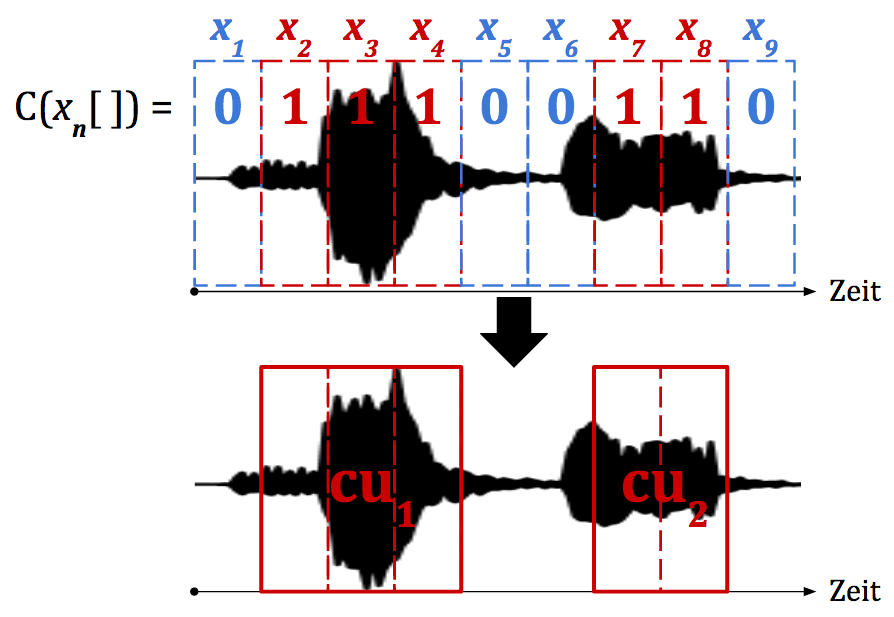
\includegraphics[width=0.6\textwidth]{bilder/cry-Unit02.png}
	\caption{Zusammenfassung als stimmhaft klassifizierter Signalfenster zu Cry-Units}
	\label{img:cryUnit}
\end{figure}

Formel \ref{eq:cry-Unit} gibt die Definition des Datentyps \emph{Cry-Unit} [$CU$]. Eine Cry-Unit wird definiert durch den Anfangszeitpunkt $start$, einen Endzeitpunkt $end$ und der Liste seiner Signalfenster $windows = \big[x_0[\;], \ldots, x_n[\;]\big]$.

\begin{equation}
CU := \quad \Big(windows = \big[x_0[\;] \; ,\ldots, x_n[\;] \big] \;, start \in Zeit \;, end \in Zeit \Big)
\label{eq:cry-Unit}
\end{equation}

Die zeitliche Dauer eine Cry-Unit $cu \in CU$ wird nach Formel \ref{eq:cry-Lambda} berechnet und mit $\lambda$ bezeichnet. Die Dauer der Pause zwischen zwei Cry-Units d($cu_i, cu_j$), wird nach Formel \ref{eq:cry-distance} berechnet. Diese Zusammenhänge werden in Abbildung \ref{img:cryUnit-details} visualisiert.\cite[S. 2]{vad_entropy}

\begin{equation}
\lambda (cu) = cu.end - cu.start
\label{eq:cry-Lambda}
\end{equation}

\begin{equation}
\text{d}(cu_i, cu_j) = cu_j.start - cu_i.end
\label{eq:cry-distance}
\end{equation}

\begin{figure}[h]
	\centering
	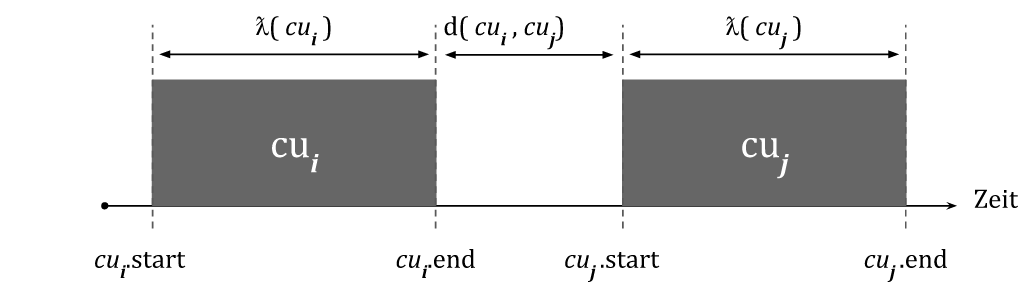
\includegraphics[width=0.9\textwidth]{bilder/newSmoothing05.png}
	\caption{Beziehung zwischen agrenzenden Cry-Units, nach \cite[S. 2]{vad_entropy}}
	\label{img:cryUnit-details}
\end{figure}

Algorithmus \ref{alg:cryUnit} zeigt in Pseudo-Code, wie auf Basis der Liste aller Signalfenster eines Signals $X_{all} = [x_0[\;] ,\ldots, x_m[\;]]$ die Liste der Cry-Units $CU_{all}$ generiert wird. Die Funktion $C(x[\;])$ ist die Klassifikations-Funktion der Signalfenster in Stille/Stimme nach Gleichung \ref{eq:cepTree01}. Die Funktion getTimeOf$(x_i[\;])$ liefert die Anfangszeitpunkt des Signalfensters $x_i[\;]$. Output des Algorithmus ist die Liste aller Cry-Units $CU_{all} = [cu_0 , \ldots, cu_l]$

\begin{algorithm}[h]
	\caption{Gruppierung von Signalfenstern zu Cry-Units}
	\label{alg:cryUnit}
	\begin{algorithmic}[1]
		\Function{turnWindowsIntoCryUnits}{$X_{all}$}
		\State $ CU_{all} \gets [\;]$
		\State $ cu\gets ([\;],0,0)$
		\For{\textbf{all} $x_i[\;] \in X_{all}$}
				\State $ c \gets C(x_i[\;])$
				\State \Comment Start of Cry-Unit
				\If {$c == 1 \wedge \text{isEmpty}(cu.windows)$}
						\State $cu\gets ([\;],0,0)$
						\State $cu.start \gets \text{getTimeOf}(x_i[\;])$
						\State $cu.windows \gets [cu.windows, x_i[\;]]$
				\EndIf
				\State \Comment Inside Cry-Unit
				\If {$c == 1 \wedge \text{ ! isEmpty}(cu.windows)$}
						\State $cu.windows \gets [cu.windows, x_i[\;]]$
				\EndIf
				\State \Comment End of Cry-Unit
				\If {$c == 0 \wedge \text{ ! isEmpty}(cu.windows)$}
						\State $cu.end \gets  getTimeOf(x_i[\;])$
						\State $CU \gets [CU, cu]$
						\State $cu.windows \gets [\;]$
				\EndIf
		\EndFor
		
		\State \Comment End last Cry-Unit by force if still open.
		\If {$\text{ ! isEmpty}(cu.windows) == 0$}
		\State $cu.end \gets  getTimeOf(X_{windows}[end])$
		\State $CU_{all} \gets [CU_{all}, cu]$
		\EndIf
		
		\Return $CU_{all}$
		
		\EndFunction
		
	\end{algorithmic}
\end{algorithm}

\section{Decision Smoothing}
\label{sec:decision_smoothing_new}

Abbildung \ref{img:beforeSmoothing} zeigt ein Audiosignal mit einem Signal-Rausch-Abstand von \SI{3}{\decibel}, bei dem die Voice Activity Detection durchgeführt wurde. Die rote Linie zeigt die tatsächliche Klassifikation und die grüne Linie die prognostizierte Klassifikation. Es ist zu sehen, dass einige False-Negatives sowie False-Positives prognostiziert wurden. Im folgenden werden drei charakteristische Varianten falsch prognostizierter Klassifikationen näher erläutert:

\begin{description}
	\item [False Negatives nach (a): ] Eine korrekt erkannte, längere Cry-Unit wird zu früh beendet. Oft werden kurz nach dem Ende einer längeren Cry-Unit sehr kurze Cry-Units erkannt, die eigentlich noch zu der längeren, vorhergehenden Cry-Unit gehören.
	\item [False Positives nach (b): ] Kurze Cry-Units werden in eigentlichen Stille-Bereichen erkannt.
	\item [False Negatives nach (c): ] Eine Cry-Unit zerfällt in zwei Cry-Units, da einige wenige Signalfenster in der Mitte als Stille erkannt wurden.
\end{description}

\begin{figure}[h]
	\centering
	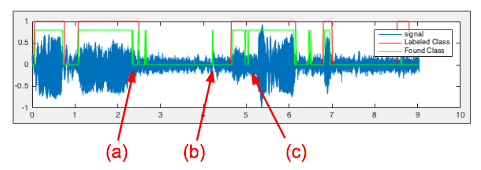
\includegraphics[width=0.7\textwidth]{bilder/smoothing02.png}
	\caption{Klassifizierung vor dem Decision Smoothing}
	\label{img:beforeSmoothing}
\end{figure}

Im Process des \textbf{Decision Smoothing} werden kontextuelle Informationen genutzt, um nachträglich False-Positives und False-Negatives zu entfernen. Es wurden dazu die von Waheed et al. \cite{vad_entropy} präsentierten Ideen verwendet. Es wurden zwei Parameter eingeführt: $\lambda_{min}$, die Mindestlänge einer akzeptierten Cry-Unit, und d$_{min}$, die Mindestlänge eines akzeptierten Stille-Segmentes. Das Decision-Smoothing wird nach den folgenden Entscheidungsregeln durchgeführt:

\textbf{Entscheidungsregeln: }\noindent\rule{0.7\linewidth}{0.3pt}
\begin{itemize}
	\item ist $\lambda (cu_{i}) \leq \lambda_{min}$ ?
	\begin{itemize}
		\item wenn $\lambda (cu_{i-1}) > \lambda_{min}$ und $d (cu_{i-1}, cu_{i}) \leq d_{min}$, dann vereinige $cu_{i}$ mit $cu_{i-1}$ $\Longrightarrow$ behebt False-Negatives des Types (a)
		\item ansonsten entferne $cu_i \Longrightarrow$ behebt False-Negatives des Types (b)
	\end{itemize}
	\item wenn $\lambda (cu_{i}) > \lambda_{min}$ und $d (cu_{i-1}, cu_{i}) \leq d_{min}$, dann vereinige $cu_{i}$ mit $cu_{i-1}$ . $\Rightarrow$ behebt False-Negatives des Types (c)
\end{itemize}
\noindent\rule{\linewidth}{0.3pt}

Die Entscheidungsregeln greifen nur auf die letzten beiden erkannten Cry-Units zu, um eine kontinuierliche Analyse zu gewährleisten. Bei einer kontinuierlichen Analyse wird dadurch die Auswertung um die Zeitdauer einer Cry-Unit verzögert, da die Entscheidungsregeln erst nach Beendigung einer Cry-Unit abgefragt werden können. Bei einer offline-Analyse können die Entscheidungsregeln vereinfacht werden, da die False-Negatives nach Typ (a) und (c) mit der selben Regel abgefragt werden können. Algorithmus \ref{alg:decisionSmoothing} zeigt in Pseudo-Code, wie das Decision-Smoothing durchgeführt wird. Input der Funktion ist die Liste aller Cry-Units $CU_{all} = [cu_0 , \ldots , cu_n]$, die durch Algorithmus \ref{alg:cryUnit} entstanden ist, sowie die Grenzwerte $\lambda_{min}$ und $d_{min}$. Der Output der Funktion ist die Liste aller Cry-Units nach dem Decision-Smoothing $CU_{smoothed}$.

\begin{algorithm}[h]
	\caption{Decision-Smoothing for VAD}
	\label{alg:decisionSmoothing}
	\begin{algorithmic}[1]
		\Function{decisionSmoothing}{$CU_{all}, \lambda_{min}, d_{min}$}
		\State $CU_{smoothed} \gets[CU_{all}[0]] $
		\State \Comment start for-loop at the \emph{second} cry-Unit!
		\For{ $i = 1 , \ldots , length(CU_{all}) - 1$}
			\State $cu_i \gets CU_{all}[i]$
			\State $cu_{i-1} \gets CU_{smoothed}[end]$
			\If{$\lambda(cu_i) > \lambda_{min}$}
			\State \Comment Accept Cry-Unit
			\If{d$(cu_{i-1},cu_{i}) > d_{min}$}
					\State $CU_{smoothed} \gets [CU_{smoothed}, cu_i] $
			\Else
					\State \Comment Erase False-Negative Type (c)
					\State $cu_i \gets \text{vereinige}(cu_i, cu_{i-1})$
					\State $CU_{smoothed} \gets [CU_{smoothed}[1:end-1], cu_i] $
			\EndIf
			\Else
			\State \Comment Erase False-Negative Type (a)
			\If{$d(cu_{i-1},cu_{i}) \leq d_{min}$ }
			\State $cu_i \gets \text{vereinige}(cu_i, cu_{i-1})$
			\State $CU_{smoothed} \gets [CU_{smoothed}[0:end-1], cu_i] $
			\Else
			\State \Comment Don't accept $cu_i$. Erases False-Positives (b)
			\EndIf
			\EndIf
		\EndFor
		
		\Return $CU_{smoothed}$
		\EndFunction
		
	\end{algorithmic}
\end{algorithm}

In verschiedenen Veröffentlichungen wurden unterschiedliche Mindestlängen von Cry-Units festgestellt. Varallyay \cite[S. 8]{cry_thesis} hat beispielsweise eine Mindestlänge von \SI{250}{\milli\second} gemessen. Der niedrigste Wert, der nach dem Wissen des Autors in einer Veröffentlichung genannt wurde, stammt von Zeskind et al. \cite[S. 325]{rythmic} und beträgt  \SI{60}{\milli\second}. Dieser Wert wurde für $\lambda_{min}$ in dieser Arbeit übernommen. Es konnten hingegen keine Veröffentlichungen gefunden werden, bei denen die geringste Pausenlänge gemessen wurde. Der Wert wurde ebenfalls mit $d_{min} = \SI{60}{\milli\second}$ bestimmt. Abbildung \ref{img:after-smoothing} zeigt das Beispielsignal vor und nach dem Decision-Smoothing. 

\begin{figure}[h]
	\centering
	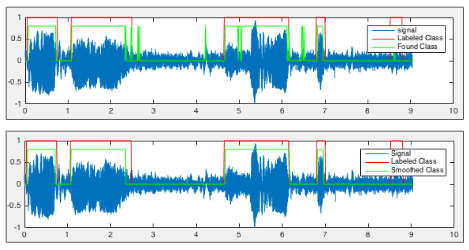
\includegraphics[width=0.8\textwidth]{bilder/smoothing04.png}
	\caption{Oben: Klassifikation vor und nach dem Decision-Smoothing. Unten: Klassifikation nach dem Decision-Smoothing.}
	\label{img:after-smoothing}
\end{figure}

\subsection{Diskussion der Voice-Activity-Detection}

In diesem Kapitel wurden verschiedene Methoden der Voice Activity Detection vorgestellt und evaluiert, wobei eine Voice Activity Detection auf Basis des Cepstrums die besten Ergebnisse erzielte. Mit Ausnahme des Decision-Smoothing werden bei diesem Ansatz jedoch keine Informationen bezüglich des zeitlichen Verlaufes mit einbezogen, da die Entscheidung über das Vorhandensein von Stimme isoliert für jedes Signalfenster gefällt wird. Schlussendlich markiert der VAD-Algorithmus eine Reihe von kurzen Signalfenstern genau dann als zusammenhängende Cry-Unit, wenn jedes Signalfenster für sich betrachtet als Lautäußerung eines Babies klassifiziert wurde. Ob jedoch die Reihenfolge der in den Signalfenstern enthaltenen Lautäußerungen Sinn macht, wird nicht betrachtet. Schneidet man beispielsweise wenige Sekunden aus der Mitte einer längeren Cry-Unit aus und konkateniert dieses Sample viele male, um eine längere Cry-Unit zu erzeugen, klingt das Ergebnis für den Menschen stark unnatürlich, wird von dem hier vorgestellten VAD-Algorithmus jedoch trotzdem als valide Cry-Unit markiert. Das Cepstrum als Feature mit der höchsten Klassifikationsgenauigkeit ist somit so zu bewerten, dass es vor allem im geringen Maße kontextuell Informationen benötigt, um eine Entscheidung über das Vorahndensein von Stimme zu fällen. Zukünftige Forschungen können an diesem Punkt ansetzen, um die Genauigkeit der VAD zu erhöhen.




